\documentclass[conference]{IEEEtran}
\IEEEoverridecommandlockouts
% The preceding line is only needed to identify funding in the first footnote. If that is unneeded, please comment it out.
\usepackage{cite}
\usepackage{amsmath,amssymb,amsfonts}
\usepackage{graphicx}
\usepackage{textcomp}
\usepackage{xcolor}
\def\BibTeX{{\rm B\kern-.05em{\sc i\kern-.025em b}\kern-.08em
    T\kern-.1667em\lower.7ex\hbox{E}\kern-.125emX}}
\title{
\vspace{1cm}
{
\includegraphics[width=0.15\textwidth]{1.jpg} \\ Finite State Machine} }
\author{Yalala Bhavani \\ Roll No: FWC22311 \\ bhavani27042003@gmail.com}
 \begin{document}
\maketitle
 \section {ABSTRACT}
 This paper explains a Finite State Machine by deconstructing the decade counter and here we verified the both incrementing decoder from $0$ to $9$ and decrementing decoder from $9$ to $0$ using arduino uno.

\section{COMPONENTS}
The required components list is given in Table: I., seven segment display is shown in Fig.1, and 7474 D-Flip Flop pin diagram is shown in Fig-2.
\vspace{0.3cm}
 \begin{table} [htbp]
\centering
\begin{tabular}{| c | c | c |} \hline
Components & Value & Quantity \\\hline
IC & 7474 & 2 \\ \hline
seven segment display & & 1\\ \hline
Arduino & UNO & 1 \\ \hline
Jumper Wires &  & 50 \\ \hline
Breadboard & & 1 \\ 
\hline
\end{tabular}
\vspace{0.3cm}
\caption{\label{tab:widgets}}
\end{table}

\begin{figure}[h]                           
\centering                                 
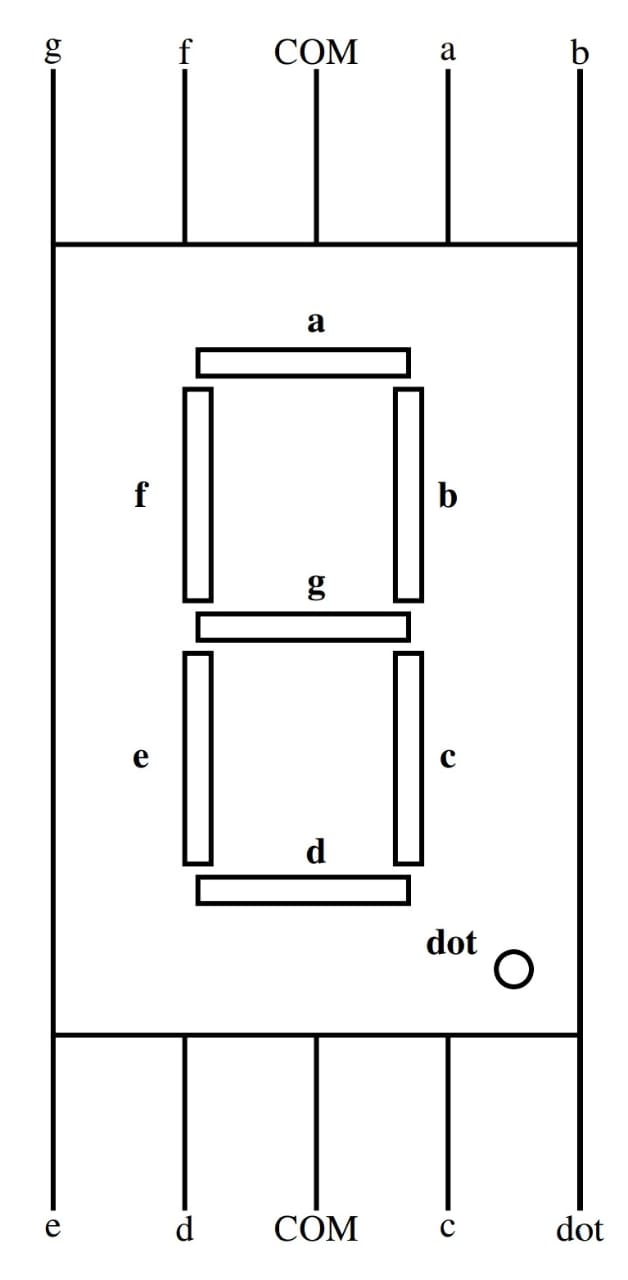
\includegraphics[width=0.15\textwidth]{2.jpg}                                           
\caption{\label{fig-1:Gates}}               
\end{figure}

\begin{figure}[h]                           
\centering                                 
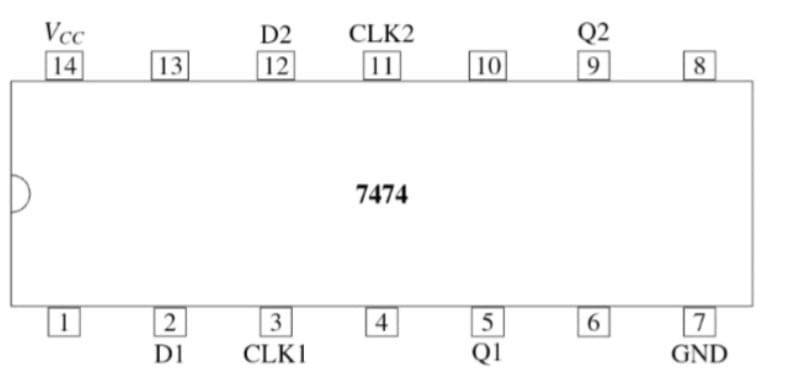
\includegraphics[width=0.2\textwidth]{3.jpg  }                                           
\caption{\label{fig-2:Gates}}               
\end{figure}

\section{PROCEDURE}


\begin{enumerate}

\item Make the connections of arduino, and two 7474 ICs according to Fig-4.
	\begin{figure}[h] 
	\centering 
	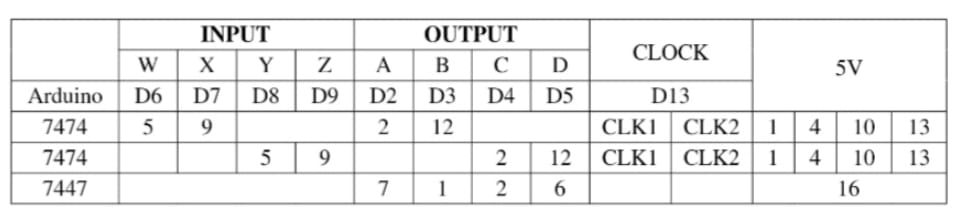
\includegraphics[width=0.3\textwidth]{4.jpg     }
	\caption{\label{fig-4:Gates}}    
\end{figure}

\item Block diagram of fsm for decade counter
\begin{figure}[h]                           
\centering                                 
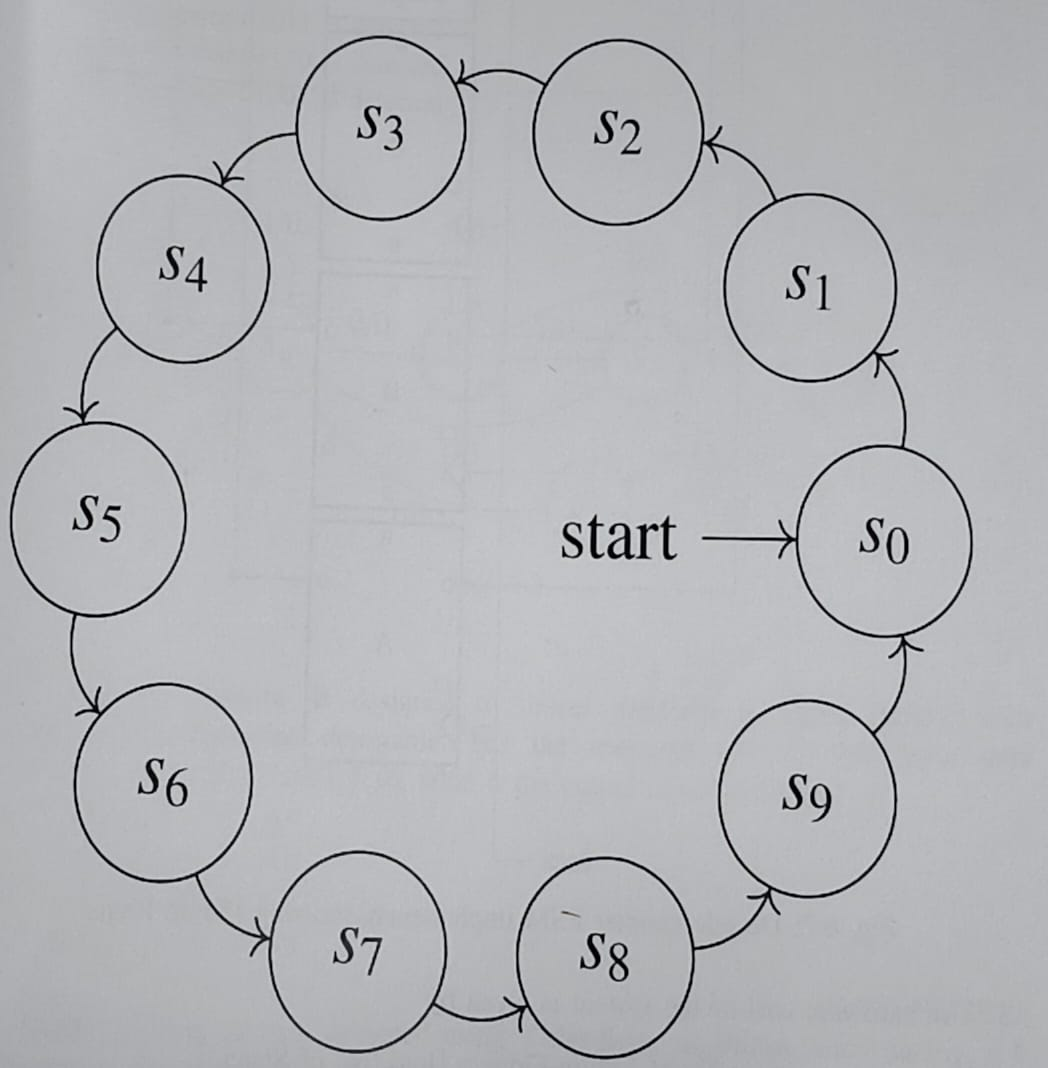
\includegraphics[width=0.2\textwidth]{5.jpg  }                                           
\caption{\label{fig-5:Gates}}               
\end{figure}



\item Block diagram of Decade Counter.

\begin{figure}[h]                           
\centering                                 
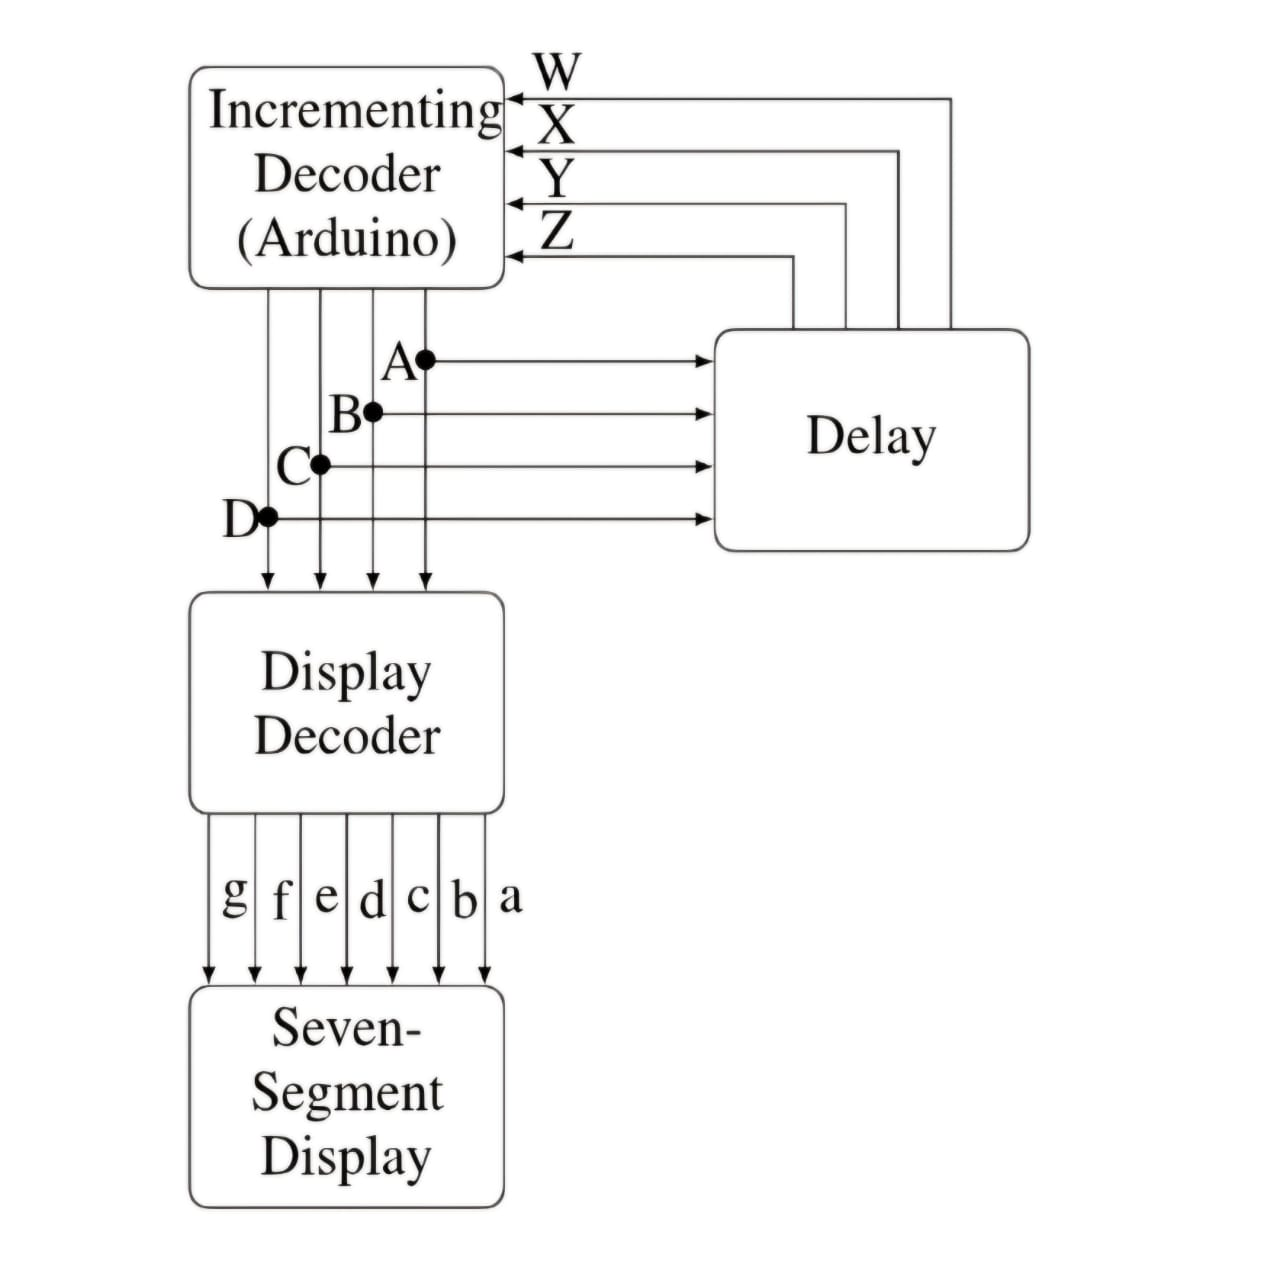
\includegraphics[width=0.2\textwidth]{6.jpg}                                           
\caption{\label{fig-5:Gates}}               
\end{figure}





\item Block diagram of Decade Counter FSM implementation using D-Flip Flops.

\begin{figure}[h]                           
\centering                                 
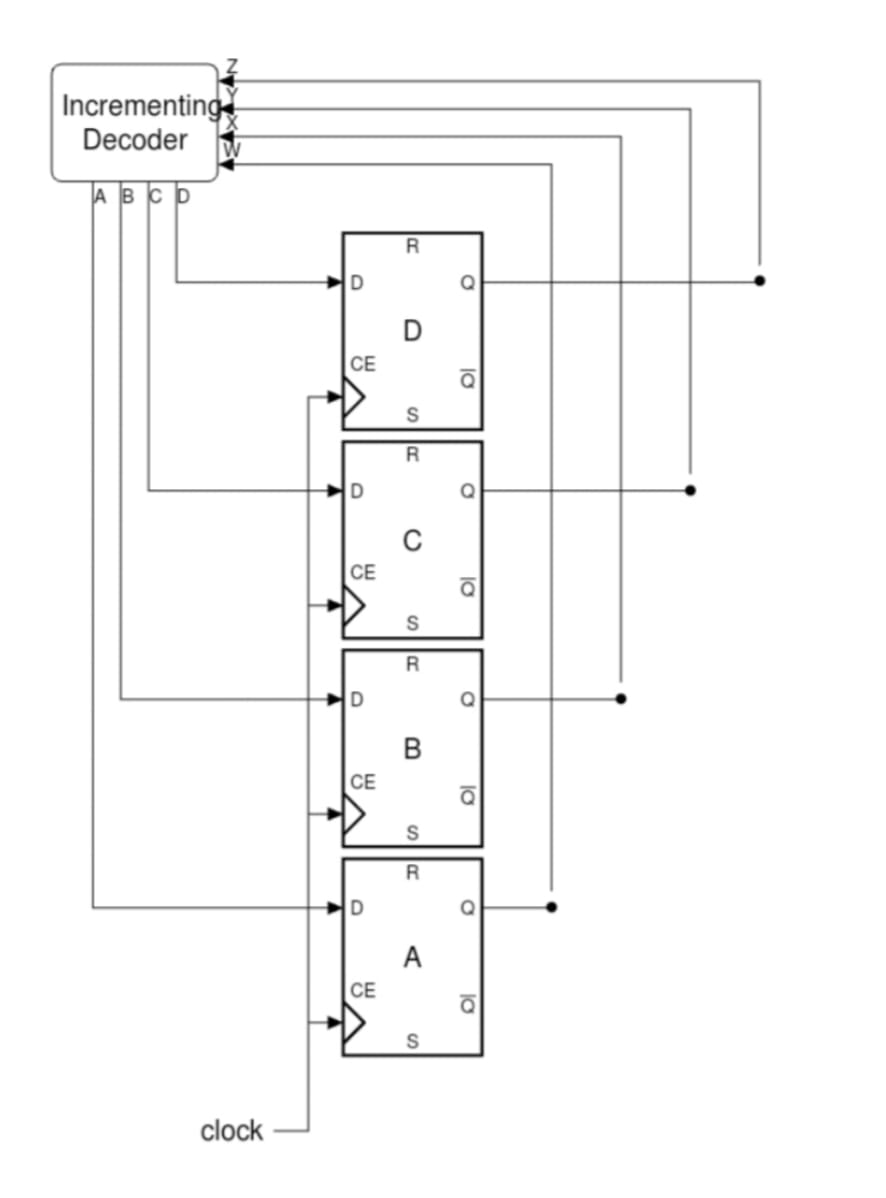
\includegraphics[width=0.3\textwidth]{7.jpg }                                           
\caption{\label{fig-5:Gates}}               
\end{figure}

\item {Truth Table for incrementing from $0$ to $9$ in seven segment display }
	\vspace{0.4cm}

\begin{table}[htbp]
    \centering
\begin{tabular}
{ | c | c | c | c | c | c | c | c | } \hline
$Z$ & $Y$ & $X$ & $W$ & $D$ & $C$ & $B$ & $A$\\\hline
0   & 0   & 0   & 0   & 0  & 0 & 0  & 1 \\
0   & 0   & 0   & 1   & 0  & 0 & 1  & 0 \\
0   & 0   & 1   & 0   & 0  & 0 & 1  & 1 \\
0   & 0   & 1   & 1   & 0  & 1 & 0  & 0 \\
0   & 1   & 0   & 0   & 0  & 1 & 0  & 1 \\  
0   & 1   & 0   & 1   & 0  & 1 & 1  & 0 \\
0   & 1   & 1   & 0   & 0  & 1 & 1  & 1 \\  
0   & 1   & 1   & 1   & 1  & 0 & 0  & 0 \\
1   & 0   & 0   & 0   & 1  & 0 & 0  & 1 \\
1   & 0   & 0   & 1   & 0  & 0 & 0  & 0 \\ \hline
\end{tabular}
\vspace{0.15cm}
\caption{\label{tab:widgets}}
\end{table}

\item {Truth Table for decrementing from $9$ to $0$ in seven segment display }

\begin{table}[htbp]
    \centering
\begin{tabular}
{ | c | c | c | c | c | c | c | c | } \hline
$Z$ & $Y$ & $X$ & $W$ & $D$ & $C$ & $B$ & $A$\\\hline
0   & 0   & 0   & 0   & 1  & 0 & 0  & 1 \\
0   & 0   & 0   & 1   & 0  & 0 & 0  & 0 \\
0   & 0   & 1   & 0   & 0  & 0 & 0  & 1 \\
0   & 0   & 1   & 1   & 0  & 0 & 1  & 0 \\
0   & 1   & 0   & 0   & 0  & 0 & 1  & 1 \\  
0   & 1   & 0   & 1   & 0  & 1 & 0  & 0 \\
0   & 1   & 1   & 0   & 0  & 1 & 0  & 1 \\  
0   & 1   & 1   & 1   & 0  & 1 & 1  & 0 \\
1   & 0   & 0   & 0   & 0  & 1 & 1  & 1 \\
1   & 0   & 0   & 1   & 1  & 0 & 0  & 0 \\ \hline
\end{tabular}
\vspace{0.15cm}
\caption{\label{tab:widgets}}
\end{table}
	
\item Execute the arduino code without any errors.
\item After upload the code into hardware setup using arduino IDE platform with hex file.
 \end{enumerate}

\section{RESULTS}
 \begin{enumerate}
	 \item Download the code given in the link below and execute them to see the output as shown in Fig.6,7. 
	 \item https://github.com/YalalaBhavani/fwc/blob/main/Fsm/main.tex
 \end{enumerate}
 \begin{figure}[h] 
	\centering 
	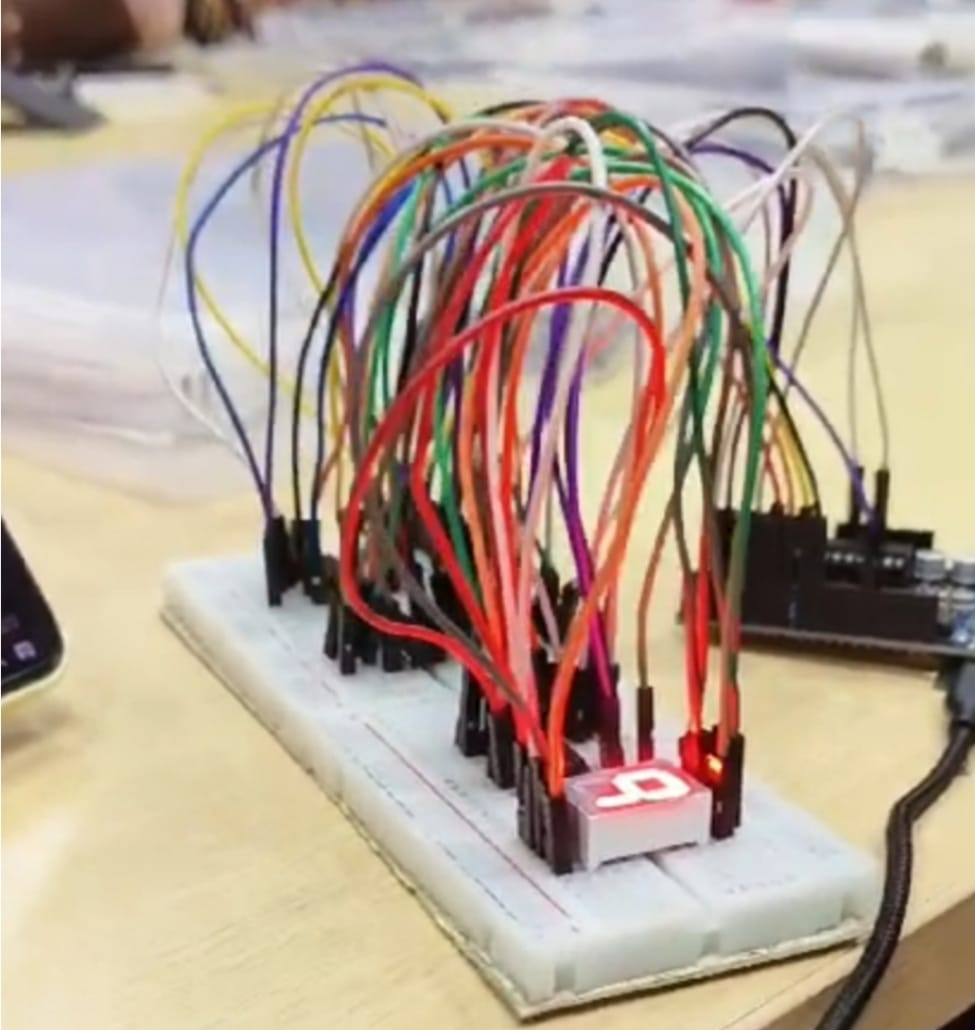
\includegraphics[width=0.25\textwidth]{8.jpg   }
	\caption{\label{fig-6:Gates}}    
\end{figure}




\section{CONCLUSION}
Hence implementation of 7474 IC Decade Couner on Seven segment dispaly using arduino UNO is done.
\end{document}
